\documentclass[12pt]{article}
\usepackage[top=0.5in, bottom=1in, left=1in, right=1in]{geometry}

%General package
\usepackage{amsmath, amsthm, amsfonts, amssymb, setspace}
\usepackage{bm}% bold math

%indentation
\usepackage[parfill]{parskip}

%Figure and references
\usepackage{subcaption}
\usepackage{tabularx,ragged2e,booktabs,caption}
\usepackage{multirow}
\usepackage{wrapfig}
\usepackage{hyperref}
\usepackage{mwe} 
\usepackage{natbib}
\bibliographystyle{abbrvnat}

%Easy List
\usepackage[ampersand]{easylist}

%Euler font
\usepackage{eulervm}
\usepackage{newpxtext}

% Tabular
\newcolumntype{C}[1]{>{\Centering}m{#1}}
\renewcommand\tabularxcolumn[1]{C{#1}}

%Stat commands
\newcommand{\E}{{\mathrm I\kern-.3em E}}
\renewcommand{\P}{{\mathrm I\kern-.3em P}}
\newcommand{\Var}{\mathrm{Var}}
\newcommand{\Cov}{\mathrm{Cov}}

\renewcommand{\vec}[1]{\mathbf{#1}}


%Mind Map
\usepackage{tikz}
\def\checkmark{\tikz\fill[scale=0.4](0,.35) -- (.25,0) -- (1,.7) -- (.25,.15) -- cycle;}


\title{Check 1D lattice gas model of 1D Protein Interaction Code}
\author{Fangzhou Xiao}
\date{20150827}
\begin{document}
	\maketitle
	\onehalfspacing

We go from small \((N,m)\) to large \((N,m)\). Exact theory is 
\begin{gather}
Z(N,m,\beta) = \sum_{k=1}^{k_{max}} Z_{cl}(N,m,k,\beta) \exp((m-k) \epsilon \beta)\\
Z_{cl}(N,m,k,\beta)= \delta_{N,m} \exp(\epsilon \beta) + \frac N k F(k, N-m)F(k,m)\\
F(k,n)=C^{n-1}_{k-1} I_{\{k\geq 1, n \geq k\}}, \hspace{1cm} k_{max} = \min(N-m+1, m)
\end{gather}

\section{\(N=m\)}

We first consider \(N=m\) case. \(k_{max} = 1\). 
\(Z_{cl}(N,N,1,\beta) = \exp (\epsilon \beta) + N F(1,0) F(1,N) = \exp (\epsilon \beta ) \) because \(F(1,0) = 0\). So 
\[
Z(N,N,\beta) = \exp(\epsilon \beta) \exp((N-1) \epsilon \beta)
= \exp(N \epsilon \beta)
\]
Therefore
\[
E = -N\epsilon 
\]
which is independent of temperature. 

\begin{figure}
	
	\begin{subfigure}{.47\textwidth}
		\centering
		\fbox{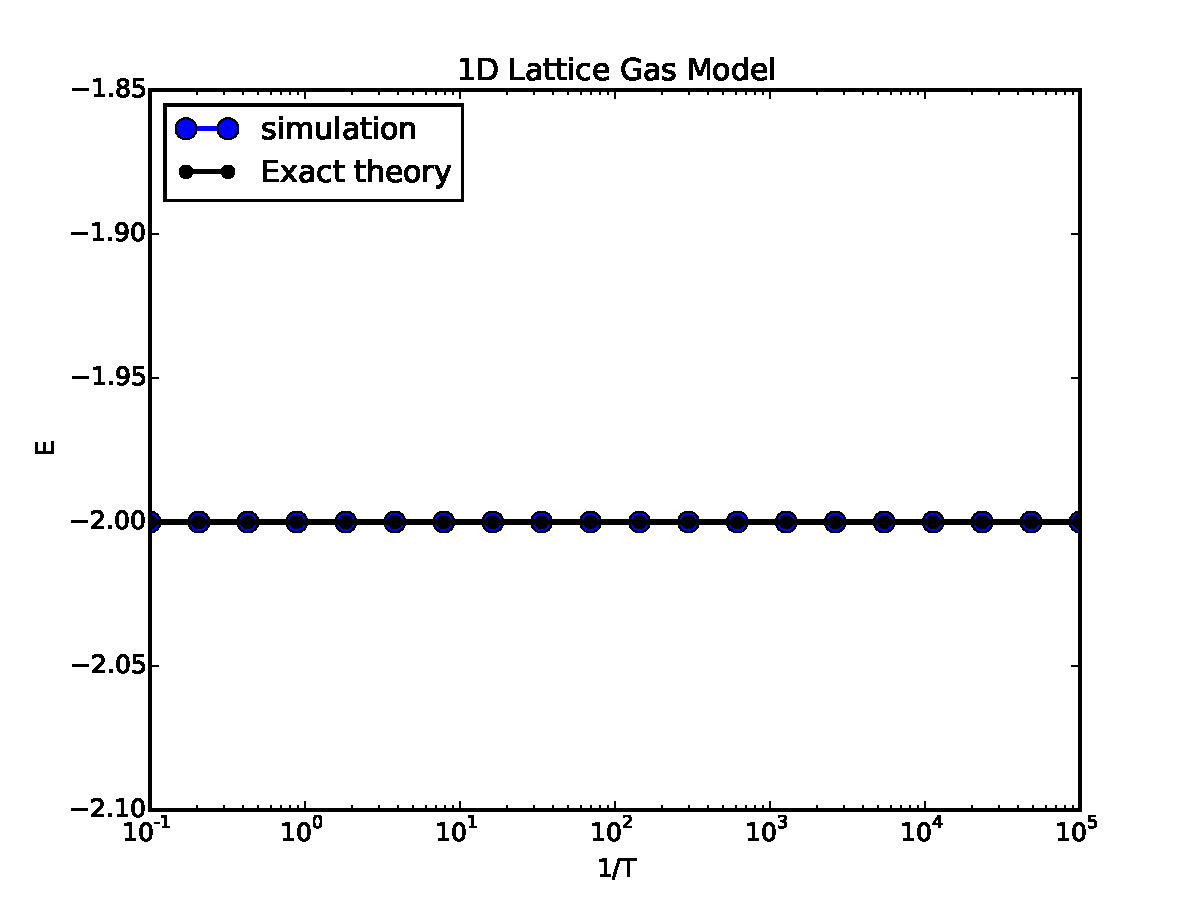
\includegraphics[width=0.9\linewidth]{1DGasTestNN2.pdf}}
		\caption{\(N=m=2\).}
		\label{fig:NN2}
	\end{subfigure}%
	\quad
	\begin{subfigure}{.47\textwidth}
		\centering
		\fbox{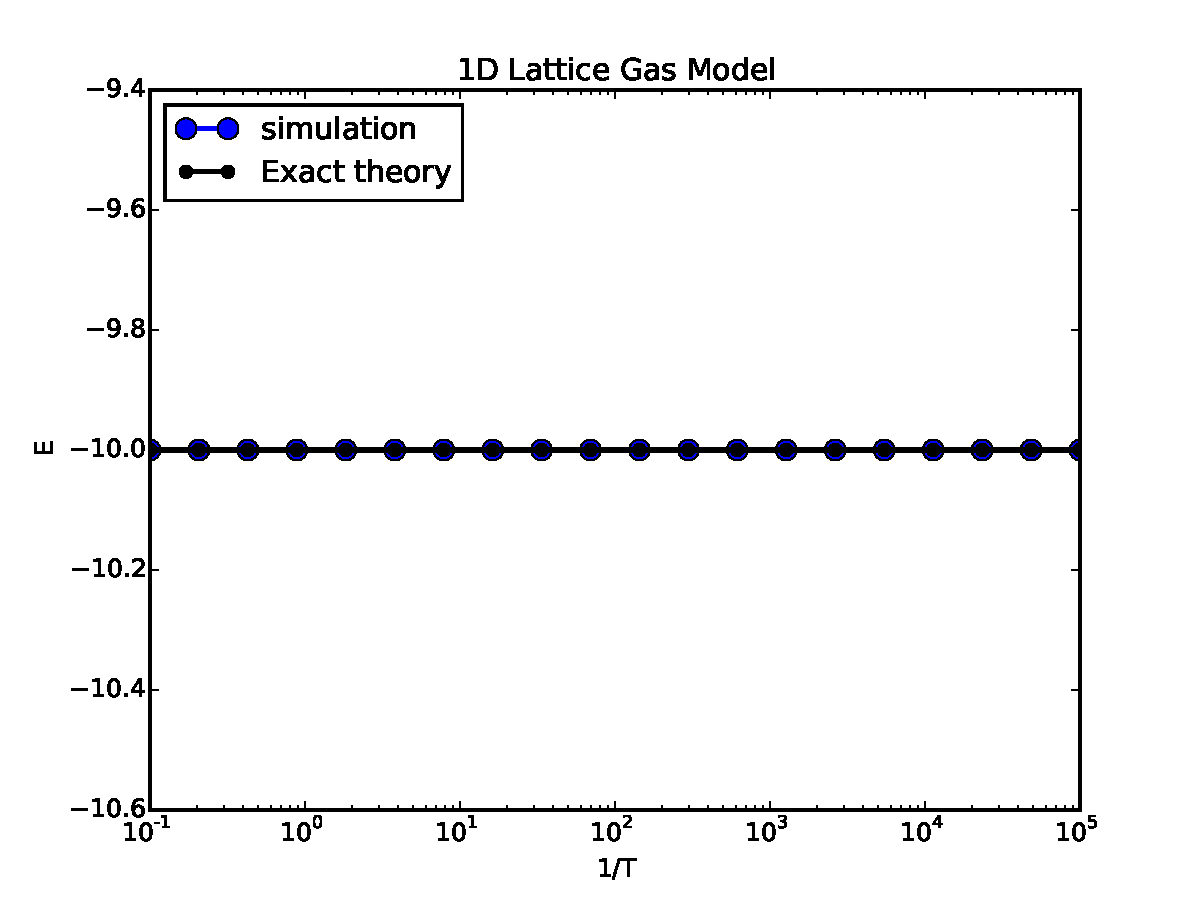
\includegraphics[width=0.9\linewidth]{1DGasTestNN10.pdf}}
		\caption{\(N=m=10\)}
		\label{fig:NN10}
	\end{subfigure}%
	
	\begin{subfigure}{.47\textwidth}
		\centering
		\fbox{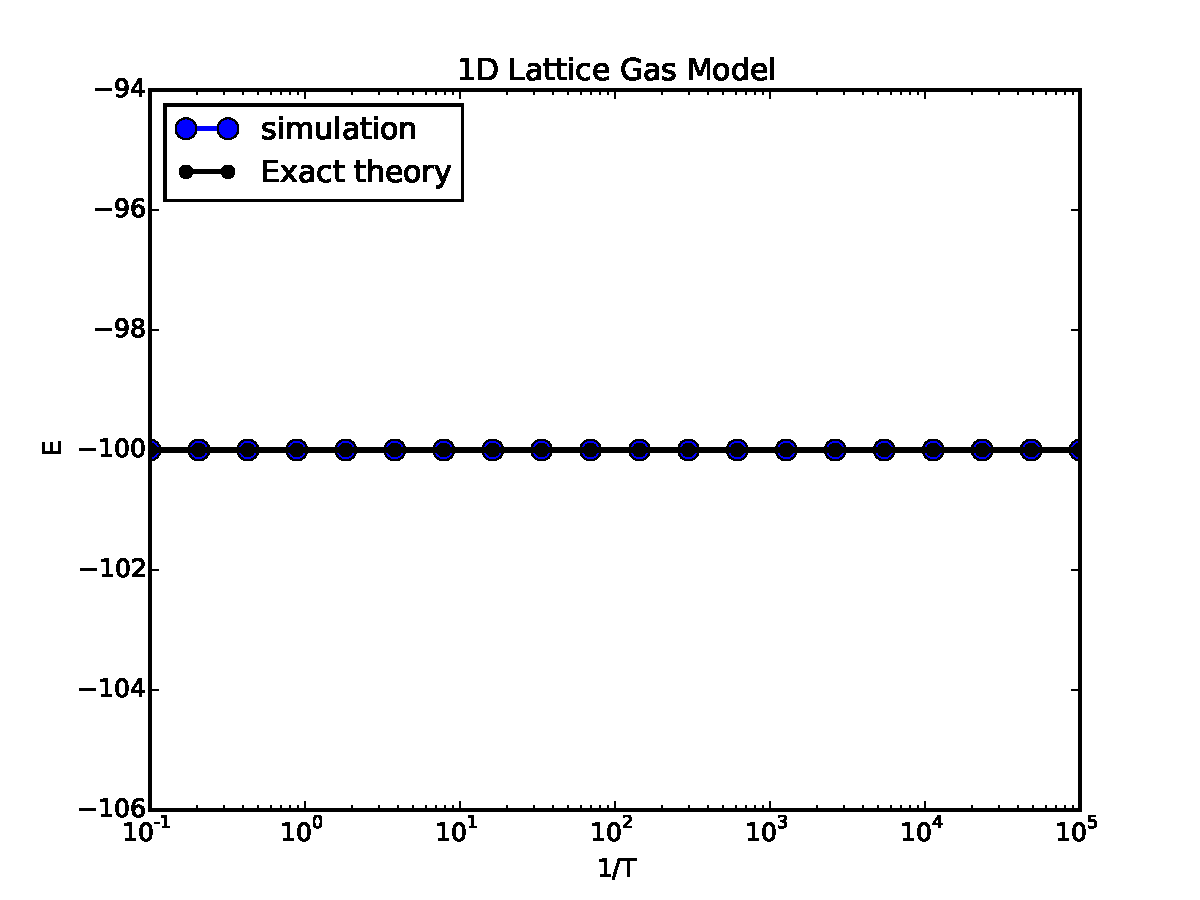
\includegraphics[width=0.9\linewidth]{1DGasTestNN100.pdf}}
		\caption{\(N=m=100\).}
		\label{fig:NN100}
	\end{subfigure}%
	
	\caption{\(N=m\) case. (obs,dur) = (150, 300) unless specified.}
	\label{fig_NN}
\end{figure}

\section{\(m \neq  N\)}
For this case. the \(\delta_{Nm}\) term disappears in \(Z_{cl}\). 
\[
Z = \sum_k Z_{cl}(k) \exp((m-k) \epsilon \beta)
\]
So energy
\[
E = \frac{ \sum_k (m-k) \epsilon Z_{cl}(k) e^{-k \epsilon \beta }} { \sum_k Z_{cl}(k) e^{-k\epsilon \beta}}
\]
where we canceled \(e^{m\epsilon \beta}\) term.

For numerical stability, we can time both the numerator and denumerator with \(\exp(\frac 1 2 k_{max} \epsilon \beta)\). But I did not implement this yet.\\

The major difference between theory and simulation is when \(T\) is large. The theory says when \(\beta \rightarrow 0\), 
\[
E = \frac {\sum_k(m-k)\epsilon Z_{cl} }  { \sum_k Z_{cl}}
\]
From computation we see for\((N,m) = (4,1)\), \(E = 0\), which agrees trivially with simulation. On the other hand, \((N,m) = (4,3)\), \(E=-2\), which also agrees completely with simulation. The latter is because no matter how we move there is always one and only one chain, of length 3.  Only \((N,m)=(4,2)\) gives non-trivial simulation results. When (obs, dur) = (150, 300), simulation and theory don't agree well at small \(\beta\). Taking (obs, dur) = (1000, 1000), we have similar agreement.... So duration isn't problem here.\\

To see whether dynamics is the problem, I then uses the alternative dynamics, i.e. not allowing hopping. (obs, dur) = (10000, 10000). Turns out this is not large enough, so I'm trying (obs, dur) = (100000, 100000). \\

From here on, I changed the temperature space to be 20 points in log scale between 1e-3 to 1e3 for better numerical stability.\\

%Decription of results of alt dynamics

Then I look at large \(N,m\) results too see whether this discrepancy disappears. (obs, dur) = (10000, 10000). \((N,m) = (400, 200)\)\\

!!!!!!!!!!!!!!!!!!!!!!!!!!!!!!!!!!!!!!!!
Eventually, as it turns out, the error in my "exact theory" implementation is forgetting "-1" in the combination function for \(F(k,n)\).....


\begin{figure}
	
	\begin{subfigure}{.47\textwidth}
		\centering
		\fbox{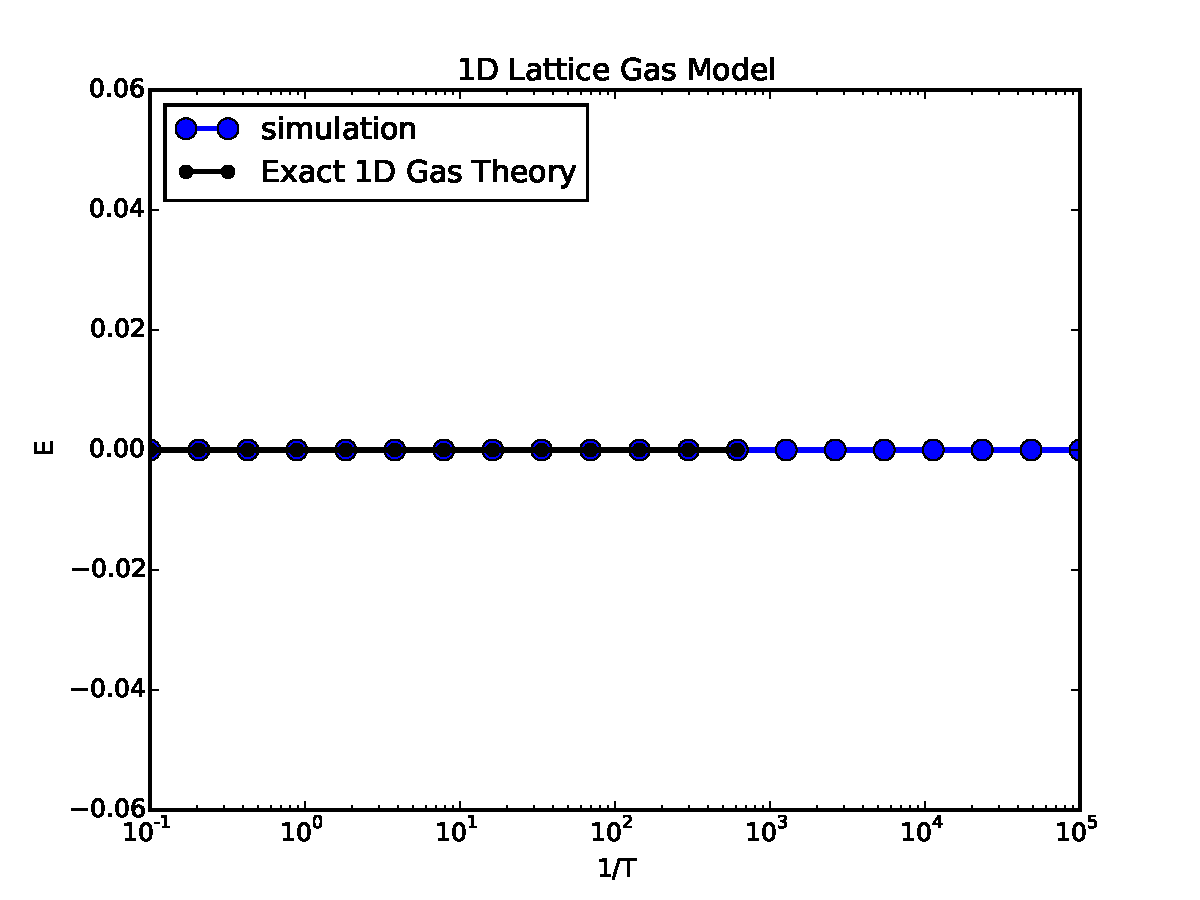
\includegraphics[width=0.9\linewidth]{1DGasTestN2m1.pdf}}
		\caption{\((N,m)=(2,1)\).}
		\label{fig:N2m1}
	\end{subfigure}%
	\quad
	\begin{subfigure}{.47\textwidth}
		\centering
		\fbox{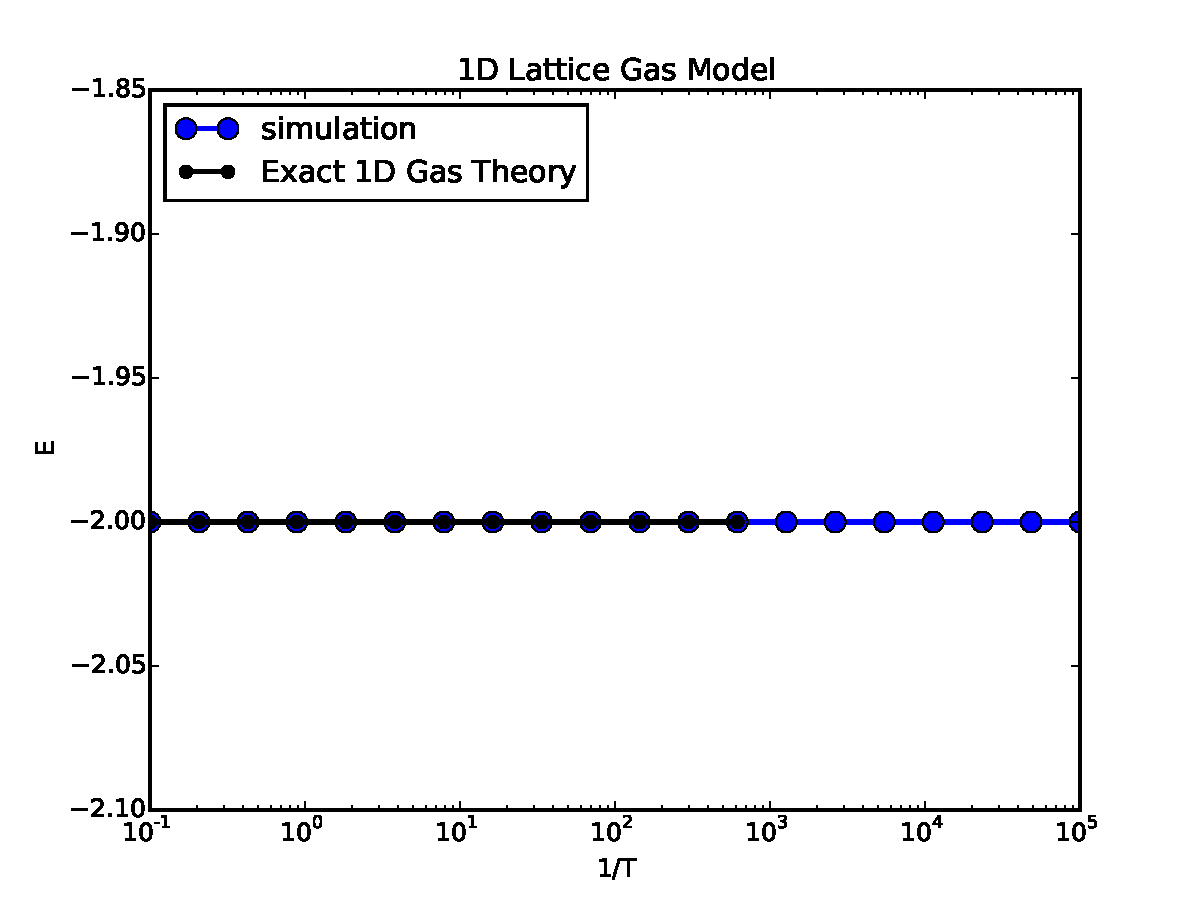
\includegraphics[width=0.9\linewidth]{1DGasTestN4m3.pdf}}
		\caption{\((N,m)=(4,3)\)}
		\label{fig:N4m3}
	\end{subfigure}%
	
	\begin{subfigure}{.47\textwidth}
		\centering
		\fbox{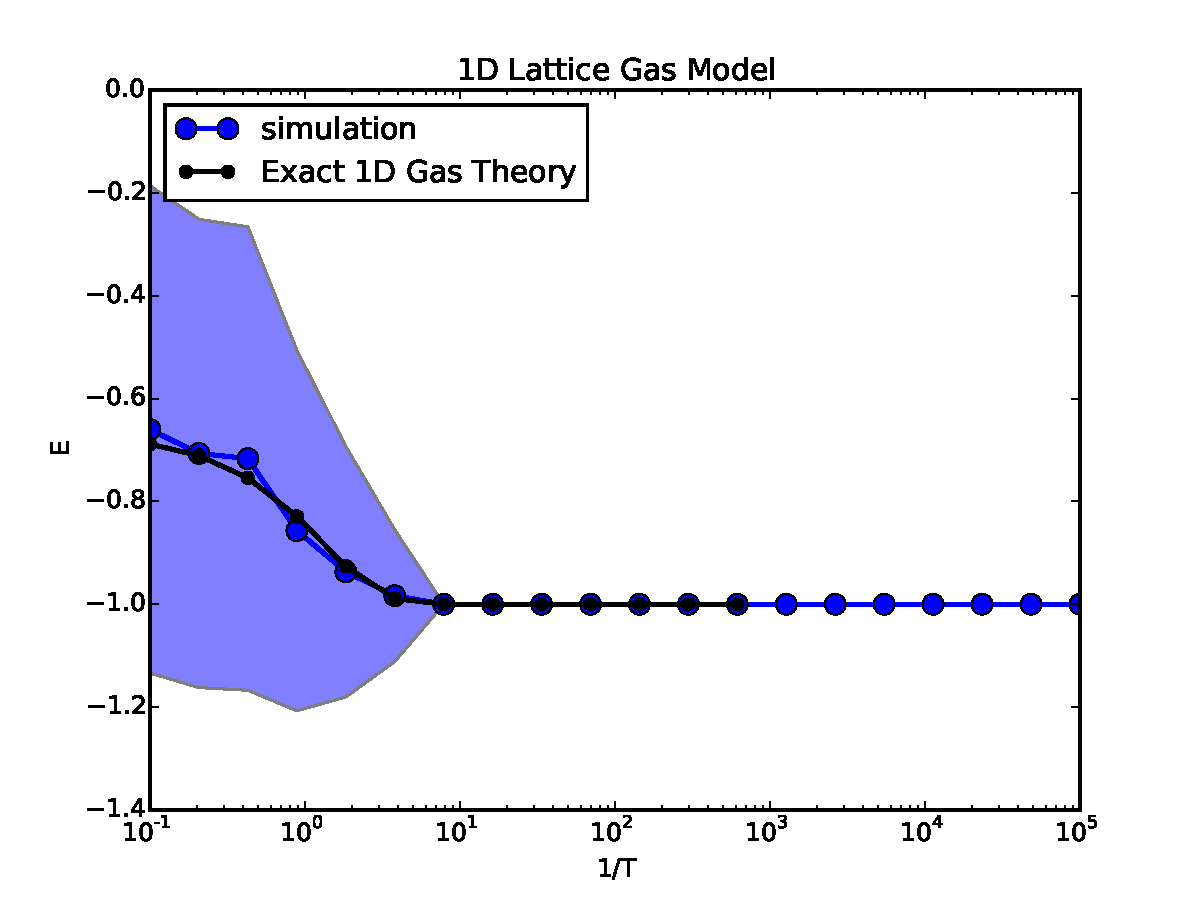
\includegraphics[width=0.9\linewidth]{1DGasTestN4m2.pdf}}
		\caption{\((N,m)=(4,2)\)}
		\label{fig:N4m2}
	\end{subfigure}%
	\quad
	\begin{subfigure}{.47\textwidth}
		\centering
		\fbox{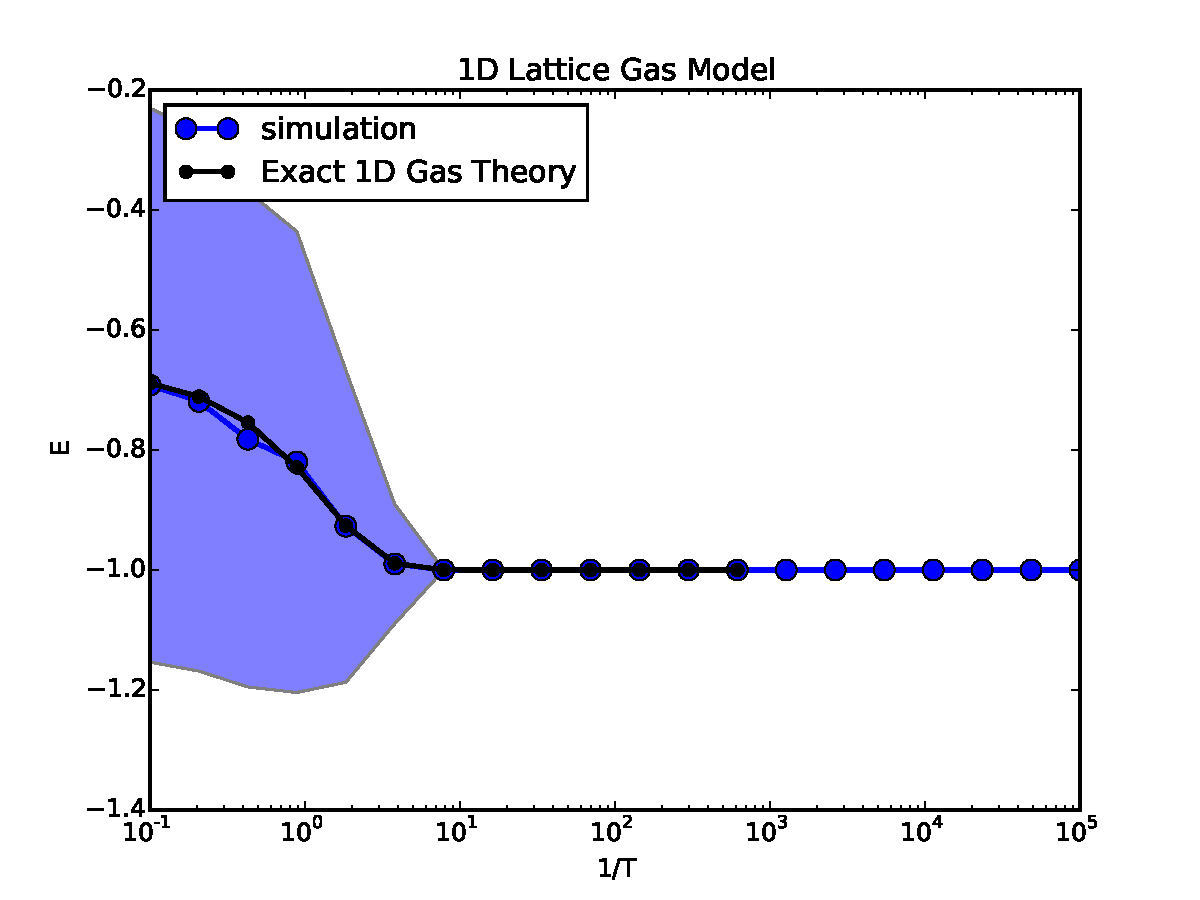
\includegraphics[width=0.9\linewidth]{1DGasTestN4m2_1e3.pdf}}
		\caption{\((N,m)=(4,2)\), (obs,dur) = (1000, 1000)}
		\label{fig:N4m3_1e3}
	\end{subfigure} %
		
	\begin{subfigure}{.47\textwidth}
		\centering
		\fbox{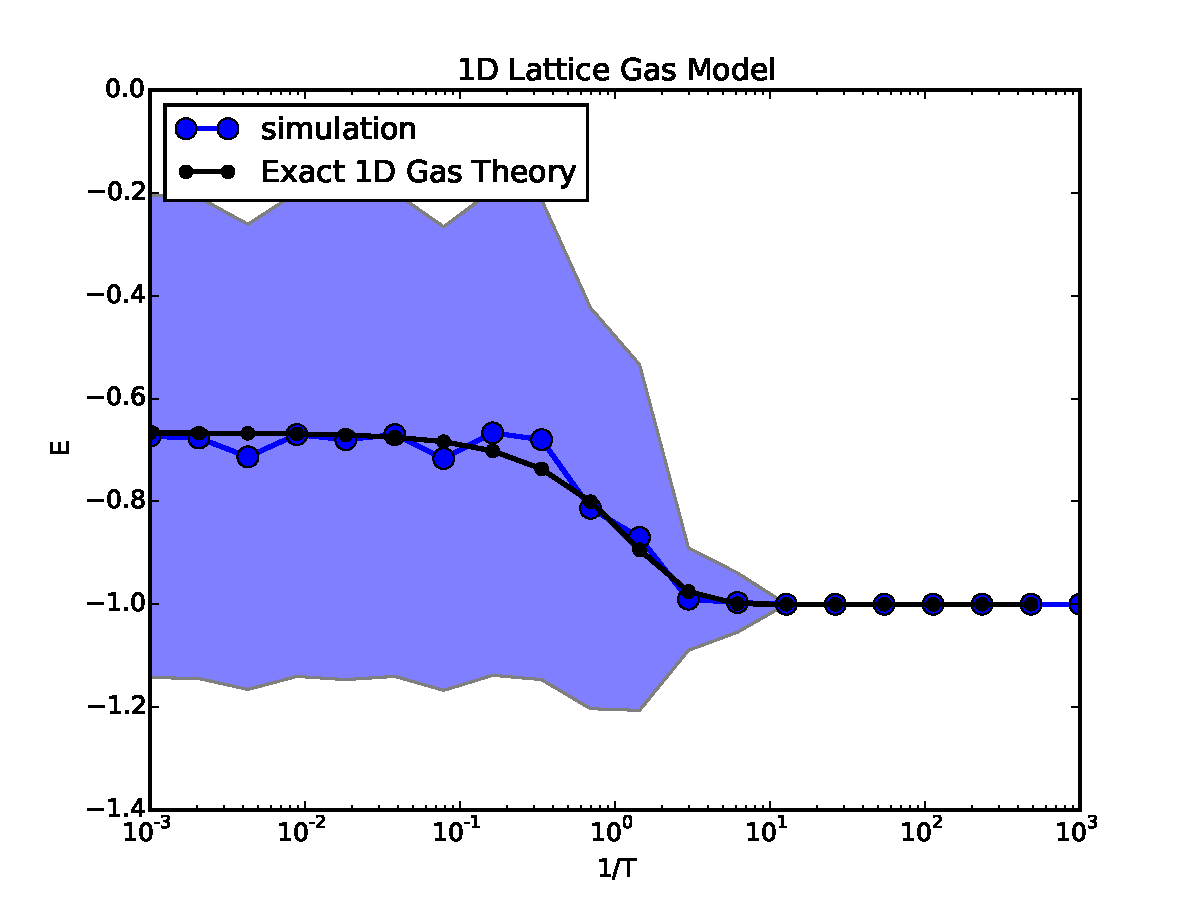
\includegraphics[width=0.9\linewidth]{1DGasTestN4m2_T.pdf}}
		\caption{\((N,m)=(4,2)\), same as \ref{fig:N4m2}, but temperature range is different.}
		\label{fig:N4m2_T}
	\end{subfigure}%
	\quad
	\begin{subfigure}{.47\textwidth}
		\centering
		\fbox{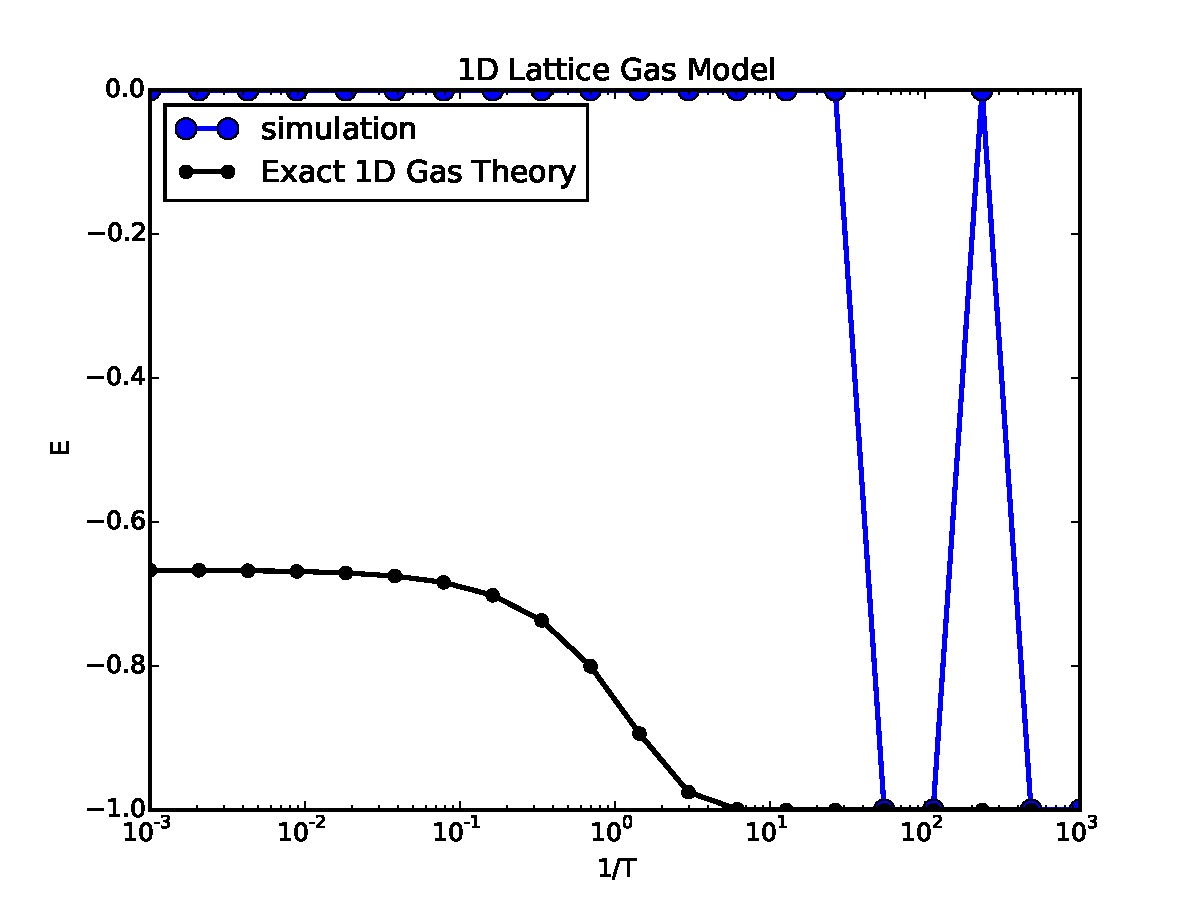
\includegraphics[width=0.9\linewidth]{1DGasTestN4m2_alt.pdf}}
		\caption{\((N,m)=(4,2)\), (obs,dur) = (10000, 10000), with no-hopping dynamics}
		\label{fig:N4m3_alt}
	\end{subfigure}%
	
	\caption{\(N\neq m\) case. (obs,dur) = (150, 300) unless specified.}
	\label{fig_Nm}
\end{figure}

\end{document}